\documentclass[pageno]{cos429}

\newcommand{\quotes}[1]{``#1''}

\widowpenalty=9999

\usepackage[normalem]{ulem}
\usepackage{amsmath}
\usepackage{algorithm2e}
\usepackage{subfig}

\DeclareMathOperator*{\argmin}{arg\,min}
\DeclareMathOperator*{\image_label}{label}

\begin{document}

\title{Robustness of Face Recognition to Image Manipulations}

\author{Cathy Chen, Zach Liu, and Lindy Zeng}
\date{}
\maketitle

\section{Motivation}
As people we can often recognize pictures of people we know even if the image has low resolution or obscures part of the face, if the camera angle resulted in a distorted image of the subject's face, or if the subject has aged or put on makeup since we last saw them. Although we seem to do this quite easily, when we think about how we accomplish this task it seems non-trivial for compute algorithms to recognize faces despite visual changes.

Moreover, computer facial recognition is highly useful. Facial recognition systems have applications ranging from airport security and suspect identification to personal device authentication and face tagging\cite{huang_face_2011}. In these real-world applications, the system must continue to recognize images of a person who looks slightly different due to the passage of time, a change in environment, or a difference in clothing.

Therefore we are interested in both the construction of face recognition algorithms and their robustness to image changes resulting from realistically plausible manipulations. Furthermore, we are curious about whether the impact of image manipulations on computer algorithms' face recognition ability mirrors impacts on humans' face recognition abilities.

\section{Goal}
In this project, we implement both face recognition algorithms and image manipulations. We then analyze the impact of each image manipulation on the recognition accuracy each algorithm, and how these influences depend on the accuracy of each algorithm on un-manipulated images.

\section{Background and Related Work}
Researchers have developed a wide variety of face recognition algorithms, such as traditional statistical methods such as PCA, more opaque methods such as deep neural networks, and proprietary systems used by governments and corporations\cite{noauthor_face_nodate}\cite{schroff_facenet:_2015}\cite{sun_meet_2017}.

Similarly, others have developed image manipulations using principles from linear algebra, such as mimicking distortions from lens distortions, as well as using neural networks, such as a system for transforming images according to specified characteristics\cite{savarese_camera_2015}\cite{upchurch_deep_2016}.

Furthermore, researchers in psychology have studied face recognition in humans. A study of "super-recognizers" (people with extraordinarily high powers of face recognition) and "developmental prosopagnosics" (people with severely impaired face recognition abilities) found that inverting images of faces impaired recognition ability more for people with stronger face recognition abilities\cite{russell_super-recognizers:_2009}. This could indicate that image manipulations tend to equalize face recognition abilities, and we investigate whether this is the case with the manipulations and face recognition algorithms we test.

\section{Methods}
To test robustness of image recognition algorithms, we implemented [TODO: INSERT NUMBER HERE] algorithms and [TODO: INSERT NUMBER HERE] image manipulations. We then tested each of the algorithms with un-manipulated images as well as images resulting from each of the manipulations. In addition to the absolute accuracy of each of these combinations, we analyzed the trend in each algorithm's performance on manipulated images to the algorithm's performance on un-manipulated images.

We describe our algorithms, manipulations, dataset, and evaluation method in the following subsections.

Our implementation is available online, as further described in the Appendix(\ref{sec:Appendix}).

\subsection{Algorithms}
\subsubsection{PCA}\hspace*{\fill} \\
We implement this algorithm according to details described in \cite{vidal_eigenfaces_2008}, based on the work of \cite{turk_eigenfaces_1991}.

We first find the principal components of the training images, and we call these principal components "eigenfaces". To classify a face, we then project the face into the space spanned by these eigenfaces and project each training face image to the same subspace. We classify the test face according to the label of the closest projected training face, where we define closeness by the Frobenius norm of the difference between the test face and each training face.

So the algorithm performs face recognition by solving $\image_label(\argmin||\Omega-\Omega_i||_2)$ where $\Omega$ is the coordinates of the test image in eigenface space and $\Omega_i$ is the coordinates of training image $i$ in eigenface space.

\subsubsection{Sparse Representation}\label{sec:sparse_representation}\hspace*{\fill} \\
We implement this algorithm according to the descriptions found in \cite{ganesh_face_2012}.

To classify a face, we first encode it as a sparse representation of the training faces. We then classify the test face according to the label whose training faces receive the greatest weight in this sparse representation.

So the algorithm performs face recognition by solving $\min||c||_1\:s.t.\:||y-\Phi c||\leq\epsilon$ and then choosing the label with the greatest weights in $c$, where $\Phi$ is the training images and $y$ is the test image.

\subsubsection{Sparse Representation with Dimension Reduction}\hspace*{\fill} \\
We implement this algorithm according to the descriptions found in \cite{ganesh_face_2012}.

We first project the test and training faces to a lower-dimension subspace using PCA, and then proceed with face classification according to the method described in section \ref{sec:sparse_representation}.
\subsubsection{Sparse Representation with Combined L1 Loss}\hspace*{\fill} \\
We implement this algorithm according to the descriptions found in \cite{ganesh_face_2012}.

We first project the test and training faces to a lower-dimension subspace using PCA, and then find a sparse encoding of the test face using a dictionary with the projected training faces in addition to the standard basis vectors. Using this sparse encoding, we perform classification as described in section \ref{sec:sparse_representation}.

So this algorithm performs face recognition by solving $\min||c||_1+||e||_1\:s.t.\:||y=\Phi c+e$, where the addition of $e$ is intended to allow the algorithm to account for small differences between images of the same person.

\subsubsection{VGG-based Classification}\hspace*{\fill} \\
We implement this algorithm based on the work and pre-trained convolutional neural network of \cite{parkhi_deep_2015}. Each image undergoes preprocessing before usage in the network. For the preprocessing, we use the deformable parts model face detector provided by \cite{parkhi_deep_2015} and crop the detected face from each of the the original images. An example of a face before and after preprocessing is shown in Figure \ref{fig:vgg_preprocessing}. We also subtract the mean values for each color channel, provided by \cite{parkhi_deep_2015}, from the images prior to using the convolutional neural network.

\begin{figure}[!htb]
\subfloat[Original Image]{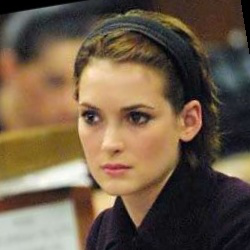
\includegraphics[width = 3in]{../figures/vgg_2.png}} 
\subfloat[Preprocessed Image]{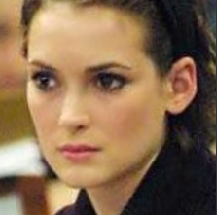
\includegraphics[width = 3in]{../figures/vgg_3.png}}
\caption{Preprocessing Demo (The face is detected and cropped from the original image)}
\label{fig:vgg_preprocessing}

\end{figure} 

Next, we translate the architecture of the VGG-based network for use with the Keras Python framework and load the pre-trained weights. We feed each face through the network, stopping at the fc-7 layer to obtain a 4,096-dimensional descriptor for each image.

For each test descriptor $w$, we calculate its cosine similarity to each training descriptor $v$. This is given by $arccos\frac{v \cdot w}{||v|| ||w||}$. The use of cosine similarity is different from the Euclidean distance methodology used in \cite{parkhi_deep_2015}, which we found to have weaker performance on our dataset. We find the nearest-$k$ neighboring training descriptors according to cosine similarity and classify the test face according to the majority vote.

\subsection{Image Manipulations}

\subsubsection{Occlusion}\hspace*{\fill} \\
The tendency for external objects to hide parts of people's faces in images motivates this manipulation. For instance, a large hat or physically faded spots on an image could hide part of someone's face, but we should still recognize the image as the same person.

We implement occlusion by selecting a region of the image and randomly resetting the pixels in this region, and show examples of occluded images in figure \ref{fig:manipulationdemo_occlusion}.

\begin{figure}[!htb]
\subfloat[Original Image]{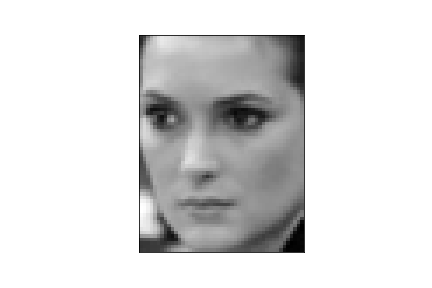
\includegraphics[width = 3in]{../figures/manipulationdemo_none}} 
\subfloat[Occluded Image]{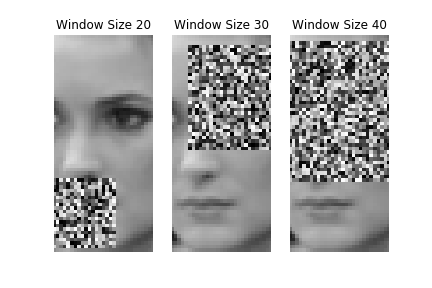
\includegraphics[width = 3in]{../figures/manipulationdemo_occlusion}}
\caption{Occlusion Demo (Window size is length of occluded region on one size)}
\label{fig:manipulationdemo_occlusion}
\end{figure}

\subsubsection{Radial Distortion}\hspace*{\fill} \\
Distortions caused by camera lenses motivate these manipulations. In particular, spherical camera lenses cause two types of radial distortion: barrel distortion disproportionately magnifies pixels closer to the optical axis and can occur with smaller focal length lenses, while pincushion distortion disproportionately magnifies pixels farther from the optical axis and can occur with larger focal length lenses \cite{drap_exact_2016}.

We mimic barrel distortion according to descriptions found in \cite{gribbon_real-time_2003}, and adapt this method for pincushion distortion as described in \cite{drap_exact_2016}.

We set $(i_0,j_0)$ as the vertical and horizontal centerline of the image, and replace the pixel at $(i,j)$ with the pixel at $(\frac{i}{1+kr^2},\frac{j}{1+kr^2})$ where $r=\sqrt{(i-i_0)^2+(j-j_0)^2}$ and $k$ is a selected parameter. A positive $k$ results in barrel distortion, while a negative $k$ results in pincushion distortion.

We provide examples of pincushion and barrel distortion for various values of $k$ in figure \ref{fig:manipulationdemo_radial}.

\begin{figure}[!htb]
\subfloat[Original Image]{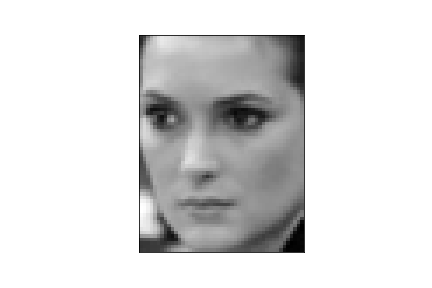
\includegraphics[width = 3in]{../figures/manipulationdemo_none}} 
\subfloat[Distorted Image]{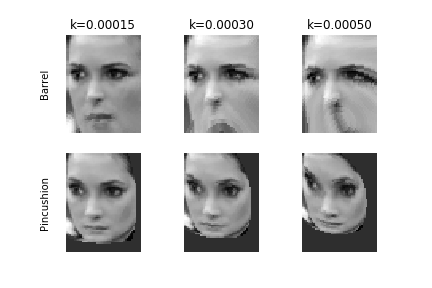
\includegraphics[width = 3in]{../figures/manipulationdemo_radial}}
\caption{Radial Distortion Demo}
\label{fig:manipulationdemo_radial}
\end{figure}

\subsubsection{Blur}\hspace*{\fill} \\
The possibility for image recognition systems to receive blurry input motivates this manipulation. We mimic blurry images by replacing each pixel by the mean value of the pixels within a pre-specified window of the replaced pixel.

We provide examples of blurred images in figure \ref{fig:manipulationdemo_blur}.
\begin{figure}[!htb]
\subfloat[Original Image]{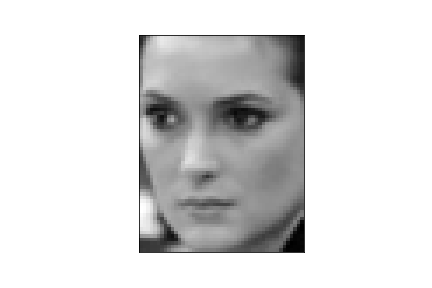
\includegraphics[width = 3in]{../figures/manipulationdemo_none}} 
\subfloat[Blurred Image]{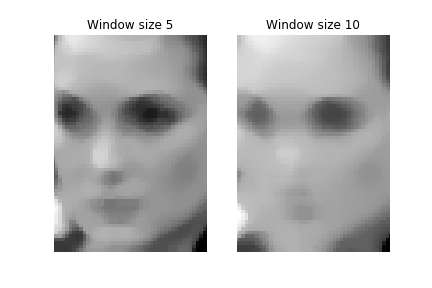
\includegraphics[width = 3in]{../figures/manipulationdemo_blur}}
\caption{Blur Distortion Demo (Window size is length of window of pixels whose mean replaces each original pixel)}
\label{fig:manipulationdemo_blur}
\end{figure}

\subsection{Deep Feature Interpretation}\hspace*{\fill} \\
TODO: DESCRIBE

\subsection{Dataset}
We use the Labeled Faces in the Wild Dataset (LFW)\cite{huang_labeled_2007}. We chose this dataset because it contains many ($13,000$) labeled images of different people ($1,680$ of whom have at least two distinct images and $62$ of whom have at least twenty distinct images). This provides sufficient training data for our experiments.

Furthermore, each of image is centered on a single face, which provides some measure of standardization between (un-manipulated) images. This allows us to control the amount and type of manipulation which we then add in our experiments, which is important because we test the robustness of algorithms to specific manipulations.

\subsection{Evaluation}
We train each algorithm using three instances of each person's face. We then evaluate each algorithm's performance according to its accuracy ($\frac{\textrm{correct predictions}}{\textrm{total predictions}}$) in recognizing faces on the test set, which includes the remaining instances of each person's face.

\section{Results and Description}
TODO: ADD RESULTS WITH VGG, DFI
TODO: ANALYZE/DESCRIBE


A deep learning approach to face recognition outperformed the statistical methods of PCA and Sparse Representation. The VGG-FACE network produced an accuracy score of over 0.98 on non-manipulated images for various values of $k$, where $k$ is the number of nearest neighboring training descriptors to compare to for each test image. We found that preprocessing the images through face detection and cropping improved performance. In addition, using cosine similarity and the nearest-$k$ neighboring heuristic, instead of Euclidean distance and the mean of the training descriptors, also improved performance. A summary of the VGG-FACE network's performance on non-manipulated images of the LFW dataset is shown in Figure \ref{fig:vgg_nonmanipulated}. 

\begin{figure}
\centering
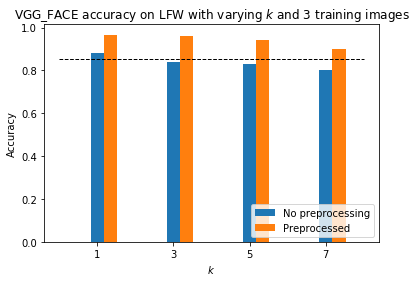
\includegraphics[scale=0.5]{../figures/vgg_1.png}
\caption{VGG-FACE Results with No Manipulations (The dotted line indicates performance with Euclidean distance and mean descriptor)}
\label{fig:vgg_nonmanipulated}
\end{figure}

\begin{figure}
\centering
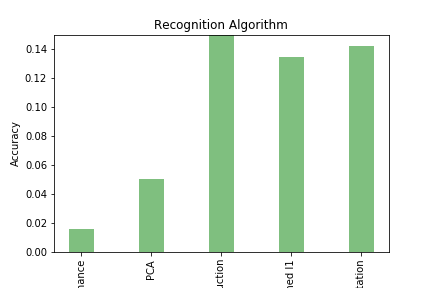
\includegraphics[scale=0.5]{../figures/results_plots/default.png}
\caption{Results with No Manipulations}
\label{fig:results_default}
\end{figure}

\begin{figure}[ht]
\centering
\subfloat{
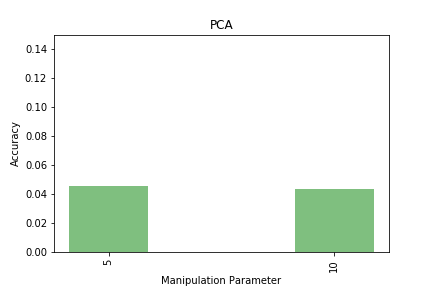
\includegraphics[width=0.5\textwidth]{../figures/results_plots/blur_PCA.png}}
\subfloat{
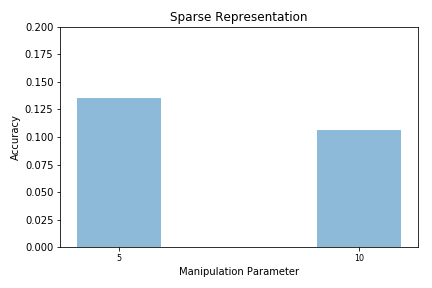
\includegraphics[width=0.5\textwidth]{../figures/results_plots/blur_SparseRepresentation.png}}
\qquad
\subfloat{
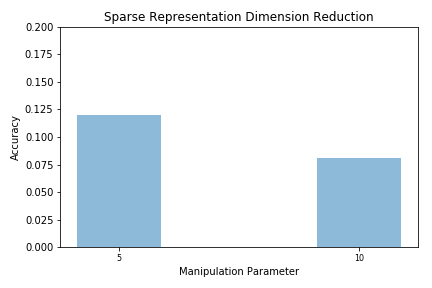
\includegraphics[width=0.5\textwidth]{../figures/results_plots/blur_SparseRepresentationDimensionReduction.png}}
\subfloat{
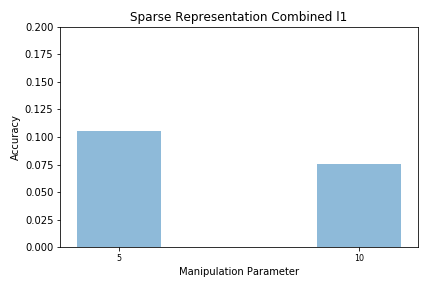
\includegraphics[width=0.5\textwidth]{../figures/results_plots/blur_SparseRepresentationCombinedl1.png}}
\caption{Test accuracy with blurred images (manipulation parameter is blur window size).}
\label{fig:results_blur}
\end{figure}

\begin{figure}[ht]
\centering
\subfloat{
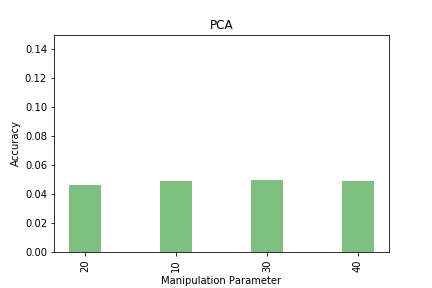
\includegraphics[width=0.5\textwidth]{../figures/results_plots/occlude_lfw_PCA.png}}
\subfloat{
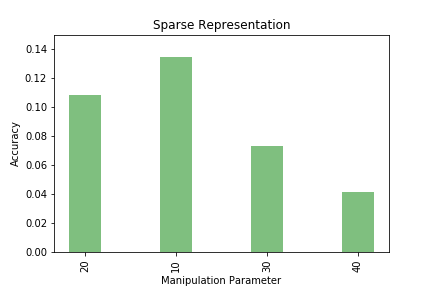
\includegraphics[width=0.5\textwidth]{../figures/results_plots/occlude_lfw_SparseRepresentation.png}}
\qquad
\subfloat{
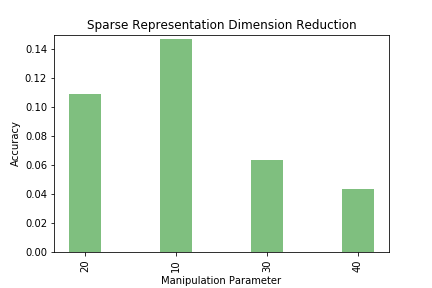
\includegraphics[width=0.5\textwidth]{../figures/results_plots/occlude_lfw_SparseRepresentationDimensionReduction.png}}
\subfloat{
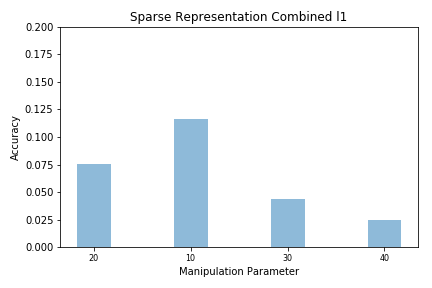
\includegraphics[width=0.5\textwidth]{../figures/results_plots/occlude_lfw_SparseRepresentationCombinedl1.png}}
\caption{Test accuracy with occluded images (manipulation parameter is occluded window size).}
\label{fig:results_occlude}
\end{figure}

\begin{figure}[ht]
\centering
\subfloat{
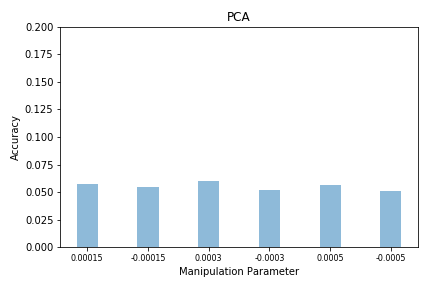
\includegraphics[width=0.5\textwidth]{../figures/results_plots/radial_distortion_PCA.png}}
\subfloat{
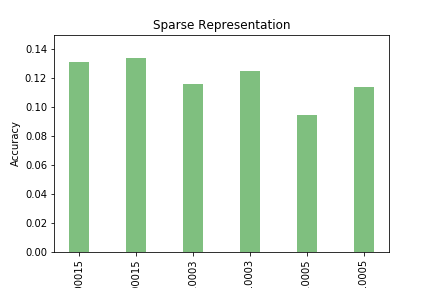
\includegraphics[width=0.5\textwidth]{../figures/results_plots/radial_distortion_SparseRepresentation.png}}
\qquad
\subfloat{
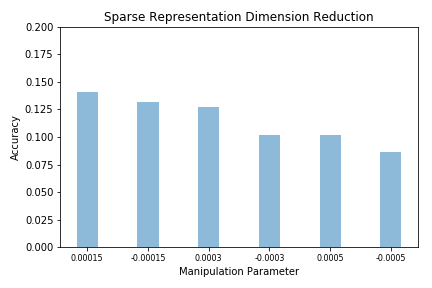
\includegraphics[width=0.5\textwidth]{../figures/results_plots/radial_distortion_SparseRepresentationDimensionReduction.png}}
\subfloat{
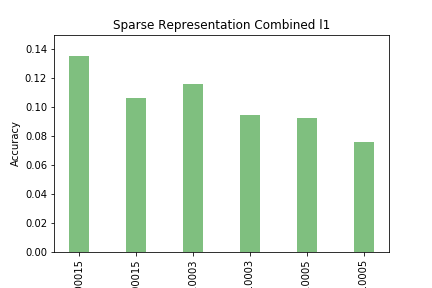
\includegraphics[width=0.5\textwidth]{../figures/results_plots/radial_distortion_SparseRepresentationCombinedl1.png}}
\caption{Test accuracy with radial distortion (manipulation parameter is $k$).}
\label{fig:results_radial}
\end{figure}
\section{Conclusion}

\bibliographystyle{plain}
\bibliography{cos429bibtex}
 
\section{Appendix}\label{sec:Appendix}
Our implementation is available \href{https://github.com/cchen23/COS429_final_project}{online}. Our implementation includes a general framework which allows the user to swap in definitions of any image manipulations and recognition algorithms, as well as modules that implement each of the manipulations and algorithms we tested.

% Maybe implementation details.
	% Dataset: at least 20 images.
% More details in README online?
\end{document}
 
